% The Clever Algorithms Project: http://www.CleverAlgorithms.com
% (c) Copyright 2011 Jason Brownlee. Some Rights Reserved. 
% This work is licensed under a Creative Commons Attribution-Noncommercial-Share Alike 2.5 Australia License.

% Name
% The algorithm name defines the canonical name used to refer to the technique, in addition to common aliases, abbreviations, and acronyms. The name is used in terms of the heading and sub-headings of an algorithm description.
\section{Gradient Descent} 
\label{sec:gradient_descent}
\index{Gradient Descent}
\index{Gradient Ascent}

% other names
% What is the canonical name and common aliases for a technique?
% What are the common abbreviations and acronyms for a technique?
\emph{Gradient Descent, Gradient Ascent.}

% Taxonomy: Lineage and locality
\subsection{Taxonomy}
\index{Steepest Descent Method}
\index{Stochastic Gradient Descent}
\index{Online Gradient Descent}
\index{Batch Gradient Descent}
% To what fields of study does a technique belong?
Gradient Descent is a first-order derivative optimization method for unconstrained nonlinear function optimization. It is called Gradient Descent because it was envisioned for function minimization. When applied to function maximization it may be referred to as Gradient Ascent. 

% What are the closely related approaches to a technique? 
Steepest Descent Search is an extension that performs a Line Search on the line of the gradient to the locate the optimum neighboring point (optimum step or steepest step).
Batch Gradient Descent is an extension where the cost function and its derivative are computed as the summed error on a collection of training examples.
Stochastic Gradient Descent (or Online Gradient Descent) is like Batch Gradient Descent except that the cost function and derivative are computed for each training example.

% Strategy: Problem solving plan
% The strategy is an abstract description of the computational model. The strategy describes the information processing actions a technique shall take in order to achieve an objective. The strategy provides a logical separation between a computational realization (procedure) and a analogous system (metaphor). A given problem solving strategy may be realized as one of a number specific algorithms or problem solving systems. The strategy description is textual using information processing and algorithmic terminology.
\subsection{Strategy}
% What is the information processing objective of a technique?
The information processing objective of the method is to locate the extremum of a function.
% What is a techniques plan of action?
This is achieved by first selecting a starting point in the search space. For a given point in the search space, the derivative of the cost function is calculated and a new point is selected down the gradient of the functions derivative at a distance of $\alpha$ (the step size parameter) from the current point. 

% Heuristics: Usage guidelines
% The heuristics element describe the commonsense, best practice, and demonstrated rules for applying and configuring a parameterized algorithm. The heuristics relate to the technical details of the techniques procedure and data structures for general classes of application (neither specific implementations not specific problem instances). The heuristics are described textually, such as a series of guidelines in a bullet-point structure.
\subsection{Heuristics}
% What are the suggested configurations for a technique?
% What are the guidelines for the application of a technique to a problem instance?

\begin{itemize}
	\item The method is limited to finding the local optimum, which if the function is convex, is also the global optimum.
	\item It is considered inefficient and slow (linear) to converge relative to modern methods. Convergence can be slow if the gradient at the optimum flattens out (gradient goes to 0 slowly). Convergence can also be slow if the Hessian is poorly conditioned (gradient changes rapidly in some directions and slower in others).
	\item The step size ($\alpha$) may be constant, may adapt with the search, and may be maintained holistically or for each dimension.
	\item The method is sensitive to initial conditions, and as such, it can be common to repeat the search process a number of times with randomly selected initial positions.
	\item If the step size parameter ($\alpha$) is too small, the search will generally take a large number of iterations to converge, if the parameter is too large can overshoot the function's optimum.
	\item Compared to non-iterative function optimization methods, gradient descent has some relative efficiencies when it comes to scaling with the number of features (dimensions).
\end{itemize}

% sample script in R
\subsection{Code Listing}
% listing
Listing~\ref{gradient_descent} provides a code listing Gradient Descent algorithm in R solving a two-dimensional nonlinear optimization function. Figure~\ref{plot:gradient_descent_result} provides a plot of the test problem with the located minimum highlighted.

% algorithm and package
The example provides a custom written \texttt{gradient\_descent()} function for locating the minimum of a two-dimensional function.
% problem
The test problem is the basin function in two-dimensions where the optimum is at $f(0)=0$ and the domain is defined as $x \in [-3,3]$. 

\lstinputlisting[firstline=7,language=r,caption={Example of Gradient Descent in R using a custom function.}, label=gradient_descent]{../src/algorithms/optimization/gradient_descent.R}

\begin{figure}[htp]
\centering
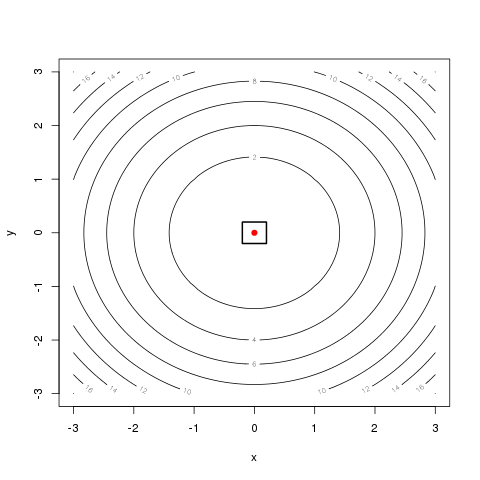
\includegraphics[scale=0.45]{a_optimization/gradient_descent_result.png}
\caption{Contour plot of the basin function with the located minimum highlighted.}
\label{plot:gradient_descent_result}
\end{figure}

% other packages
Another other packages that provides an implementation of Gradient Descent include \texttt{animation}. The \texttt{gsl} package in the \texttt{multimin()} function provides an implementation of Steepest Descent that makes use of the GNU Scientific Library \cite{Hankin2011}.

% References: Deeper understanding
% The references element description includes a listing of both primary sources of information about the technique as well as useful introductory sources for novices to gain a deeper understanding of the theory and application of the technique. The description consists of hand-selected reference material including books, peer reviewed conference papers, journal articles, and potentially websites. A bullet-pointed structure is suggested.
\subsection{References}
% What are the primary sources for a technique?
% What are the suggested reference sources for learning more about a technique?

% primary sources
\subsubsection{Primary Sources}
% seminal
The method of Steepest Descent can be traced back to Cauchy in 1847 who proposed the use of the gradient to minimize a system of simultaneous equations \cite{Cauchy1847} (French). Gradient Descent may be considered a relaxation of this original method.
% early extensions
There have been many extensions of the method. Curry provides an early extension that seeks the first stable point on the line following the gradient \cite{Curry1944}. Spang provided a good early review of minimization methods providing context for Steepest Descent \cite{Spang1962}.

% more info
\subsubsection{More Information}
Gradient Descent is a cornerstone of Machine Learning methods and is the go-to method for optimizing the cost or loss functions at the core of many modern algorithms. As such, a description can be found in any good text on Artificial Intelligence, Machine Learning, or Numerical Methods.


% END
